\documentclass[portrait,final,a1paper,fontscale=0.277]{baposter}

\usepackage{calc}
\usepackage{graphicx}
\usepackage{amsmath}
\usepackage{amssymb}
\usepackage{relsize}
\usepackage{multirow}
\usepackage{rotating}
\usepackage{bm}
\usepackage{enumitem}
\usepackage{url}
\usepackage{booktabs}
\usepackage{subfigure}

\usepackage{graphicx}
\usepackage{multicol}

%\usepackage{times}
%\usepackage{helvet}
%\usepackage{bookman}
\usepackage{palatino}

\newcommand{\captionfont}{\footnotesize}

\graphicspath{{images/}{../images/}}
\usetikzlibrary{calc}


\newcommand{\Matrix}[1]{\begin{bmatrix} #1 \end{bmatrix}}
\newcommand{\Vector}[1]{\begin{pmatrix} #1 \end{pmatrix}}

\newcommand*{\norm}[1]{\mathopen\| #1 \mathclose\|}% use instead of $\|x\|$
\newcommand*{\abs}[1]{\mathopen| #1 \mathclose|}% use instead of $\|x\|$
\newcommand*{\normLR}[1]{\left\| #1 \right\|}% use instead of $\|x\|$

\newcommand*{\SET}[1]  {\ensuremath{\mathcal{#1}}}
\newcommand*{\FUN}[1]  {\ensuremath{\mathcal{#1}}}
\newcommand*{\MAT}[1]  {\ensuremath{\boldsymbol{#1}}}
\newcommand*{\VEC}[1]  {\ensuremath{\boldsymbol{#1}}}
\newcommand*{\CONST}[1]{\ensuremath{\mathit{#1}}}

\DeclareMathOperator*{\argmax}{arg\,max}
\DeclareMathOperator*{\diag}{diag}
\DeclareMathOperator*{\argmin}{arg\,min}
\DeclareMathOperator*{\vectorize}{vec}
\DeclareMathOperator*{\reshape}{reshape}

%\font\dsfnt=dsrom12

\newcommand{\SNN}{\ensuremath{\mathbb N}}
\newcommand{\SRR}{\ensuremath{\mathbb R}}
\newcommand{\SZZ}{\ensuremath{\mathbb Z}}
%-----------------------------------------------------------------------------
% Matrices of the shape model
\renewcommand{\a}{\VEC\alpha}
\renewcommand{\v}{\VEC v}
\renewcommand{\l}{\VEC l}
\newcommand*{\m}{\VEC{\mu}}
\newcommand*{\M}{\MAT{M}}
\renewcommand*{\P}{\MAT{\Pi}}

%\newcommand{\J}{\SET J}
\newcommand{\J}{\SET{P}}
\newcommand{\Active}{\mathcal{A}}
\newcommand{\Selection}{\mathbf{S}}
\newcommand{\AllSelections}{\mathfrak{S}}
\newcommand{\Params}{\VEC\Theta}

%%%%%%%%%%%%%%%%%%%%%%%%%%%%%%%%%%%%%%%%%%%%%%%%%%%%%%%%%%%%%%%%%%%%%%%%%%%%%%%%
%%%% Some math symbols used in the text
%%%%%%%%%%%%%%%%%%%%%%%%%%%%%%%%%%%%%%%%%%%%%%%%%%%%%%%%%%%%%%%%%%%%%%%%%%%%%%%%

%%%%%%%%%%%%%%%%%%%%%%%%%%%%%%%%%%%%%%%%%%%%%%%%%%%%%%%%%%%%%%%%%%%%%%%%%%%%%%%%
% Multicol Settings
%%%%%%%%%%%%%%%%%%%%%%%%%%%%%%%%%%%%%%%%%%%%%%%%%%%%%%%%%%%%%%%%%%%%%%%%%%%%%%%%
\setlength{\columnsep}{1.5em}
\setlength{\columnseprule}{0mm}

%%%%%%%%%%%%%%%%%%%%%%%%%%%%%%%%%%%%%%%%%%%%%%%%%%%%%%%%%%%%%%%%%%%%%%%%%%%%%%%%
% Save space in lists. Use this after the opening of the list
%%%%%%%%%%%%%%%%%%%%%%%%%%%%%%%%%%%%%%%%%%%%%%%%%%%%%%%%%%%%%%%%%%%%%%%%%%%%%%%%
\newcommand{\compresslist}{%
\setlength{\itemsep}{1pt}%
\setlength{\parskip}{0pt}%
\setlength{\parsep}{0pt}%
}

%%%%%%%%%%%%%%%%%%%%%%%%%%%%%%%%%%%%%%%%%%%%%%%%%%%%%%%%%%%%%%%%%%%%%%%%%%%%%%
%%% Begin of Document
%%%%%%%%%%%%%%%%%%%%%%%%%%%%%%%%%%%%%%%%%%%%%%%%%%%%%%%%%%%%%%%%%%%%%%%%%%%%%%

\begin{document}

%%%%%%%%%%%%%%%%%%%%%%%%%%%%%%%%%%%%%%%%%%%%%%%%%%%%%%%%%%%%%%%%%%%%%%%%%%%%%%
%%% Here starts the poster
%%%---------------------------------------------------------------------------
%%% Format it to your taste with the options
%%%%%%%%%%%%%%%%%%%%%%%%%%%%%%%%%%%%%%%%%%%%%%%%%%%%%%%%%%%%%%%%%%%%%%%%%%%%%%
% Define some colors

\definecolor{lightblue}{rgb}{0.2,0.2,1}
\definecolor{lightestblue}{rgb}{0.7,0.7,1}
\definecolor{darkblue}{rgb}{0,0,0.3}

\hyphenation{resolution occlusions}
%%
\begin{poster}%
  % Poster Options
  {
  % Show grid to help with alignment
  grid=false,
  % Column spacing
  columns=2,
  colspacing=1em,
  % Color style
  bgColorOne=lightestblue,
  bgColorTwo=white,
  borderColor=darkblue,
  headerColorOne=darkblue,
  headerColorTwo=lightblue,
  headerFontColor=white,
  boxColorOne=lightestblue,
  boxColorTwo=lightblue,
  % Format of textbox
  textborder=faded,
  % Format of text header
  eyecatcher=true,
  headerborder=closed,
  headerheight=0.2\textheight,
%  textfont=\sc, An example of changing the text font
  headershape=roundedright,
  headershade=shadelr,
  headerfont=\Large\bf\textsc, %Sans Serif
  textfont={\setlength{\parindent}{1.5em}},
  boxshade=plain,
%  background=shade-tb,
  background=plain,
  linewidth=2pt
  }
  % Eye Catcher
 {} 
  % Title
  {\bf\textsc{NovelSearch: The Right Way to Download Novels}\vspace{0.5em}}
  % Authors
  {\textsc{Jiahui Chen, Jianfei Chen, and Shumei Zhang\\Tsinghua University\\{chenjf10@mails.tsinghua.edu.cn}}}
  % University logo
  {% The makebox allows the title to flow into the logo, this is a hack because of the L shaped logo.
    
\includegraphics[height=10.5em]{images/logo.png}
  }

%%%%%%%%%%%%%%%%%%%%%%%%%%%%%%%%%%%%%%%%%%%%%%%%%%%%%%%%%%%%%%%%%%%%%%%%%%%%%%
%%% Now define the boxes that make up the poster
%%%---------------------------------------------------------------------------
%%% Each box has a name and can be placed absolutely or relatively.
%%% The only inconvenience is that you can only specify a relative position 
%%% towards an already declared box. So if you have a box attached to the 
%%% bottom, one to the top and a third one which should be in between, you 
%%% have to specify the top and bottom boxes before you specify the middle 
%%% box.
%%%%%%%%%%%%%%%%%%%%%%%%%%%%%%%%%%%%%%%%%%%%%%%%%%%%%%%%%%%%%%%%%%%%%%%%%%%%%%
    %
    % A coloured circle useful as a bullet with an adjustably strong filling
    \newcommand{\colouredcircle}{%
      \tikz{\useasboundingbox (-0.2em,-0.32em) rectangle(0.2em,0.32em); \draw[draw=black,fill=lightblue,line width=0.03em] (0,0) circle(0.18em);}}

%%%%%%%%%%%%%%%%%%%%%%%%%%%%%%%%%%%%%%%%%%%%%%%%%%%%%%%%%%%%%%%%%%%%%%%%%%%%%%
  \headerbox{Problem}{name=problem,column=0,row=0}{
%%%%%%%%%%%%%%%%%%%%%%%%%%%%%%%%%%%%%%%%%%%%%%%%%%%%%%%%%%%%%%%%%%%%%%%%%%%%%%
Downloading novels online is a emerging requirement for modern Chinese netizens, such operation should be done as easy as possible on both computer and mobile devices. Current popular solutions including Google search a novel site, read it online, or Sina iAsk require follow many links to find the novel, and not friendly to mobile devices. NovelSearch is a elegant solution to this problem.
 }

%%%%%%%%%%%%%%%%%%%%%%%%%%%%%%%%%%%%%%%%%%%%%%%%%%%%%%%%%%%%%%%%%%%%%%%%%%%%%%
  \headerbox{Features}{name=contribution,column=0,below=problem}{
%%%%%%%%%%%%%%%%%%%%%%%%%%%%%%%%%%%%%%%%%%%%%%%%%%%%%%%%%%%%%%%%%%%%%%%%%%%%%%
Downloading a novel from NovelSearch only requires one input and one click:
%\begin{tabular}

%\end{tabular}
{\centering
\parbox[c]{0.49\linewidth}{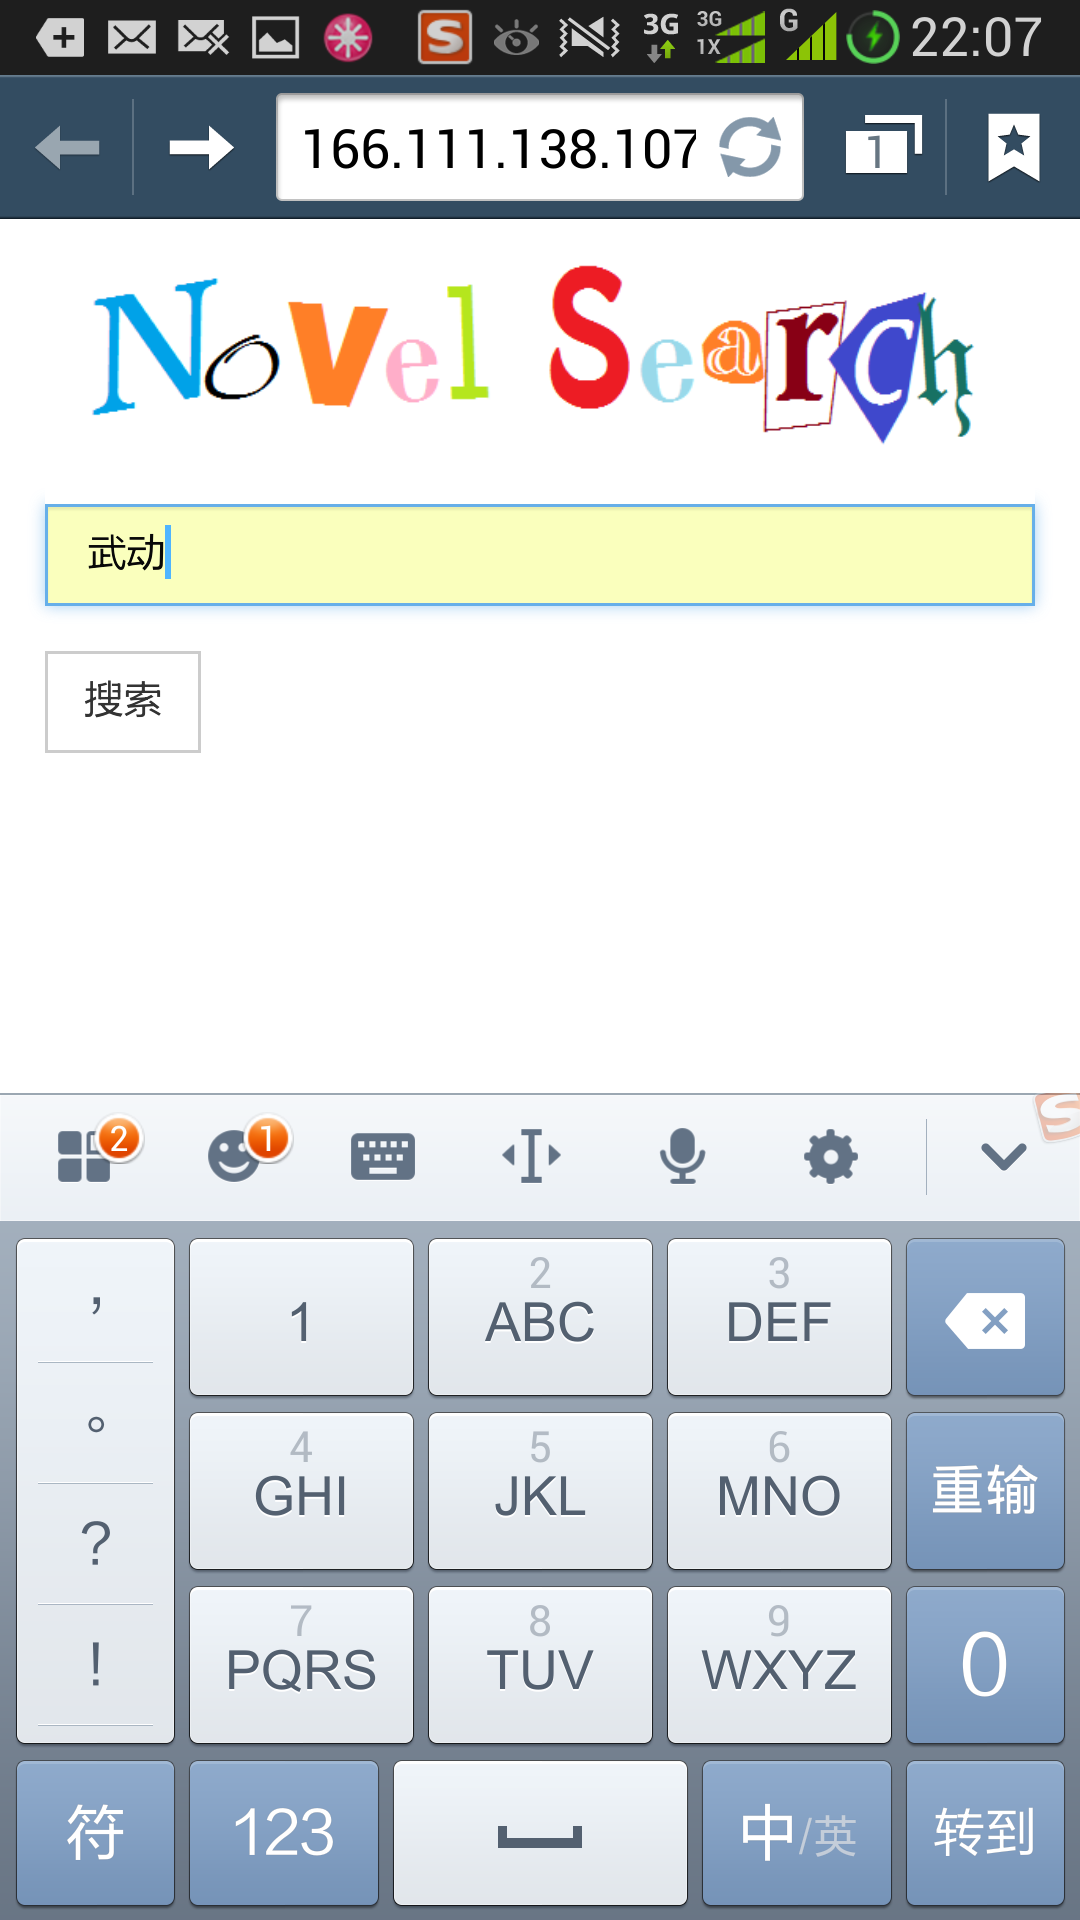
\includegraphics[width=\linewidth]{images/search.png}\\\centering{(a) Input the name of the novel.}}
\parbox[c]{0.49\linewidth}{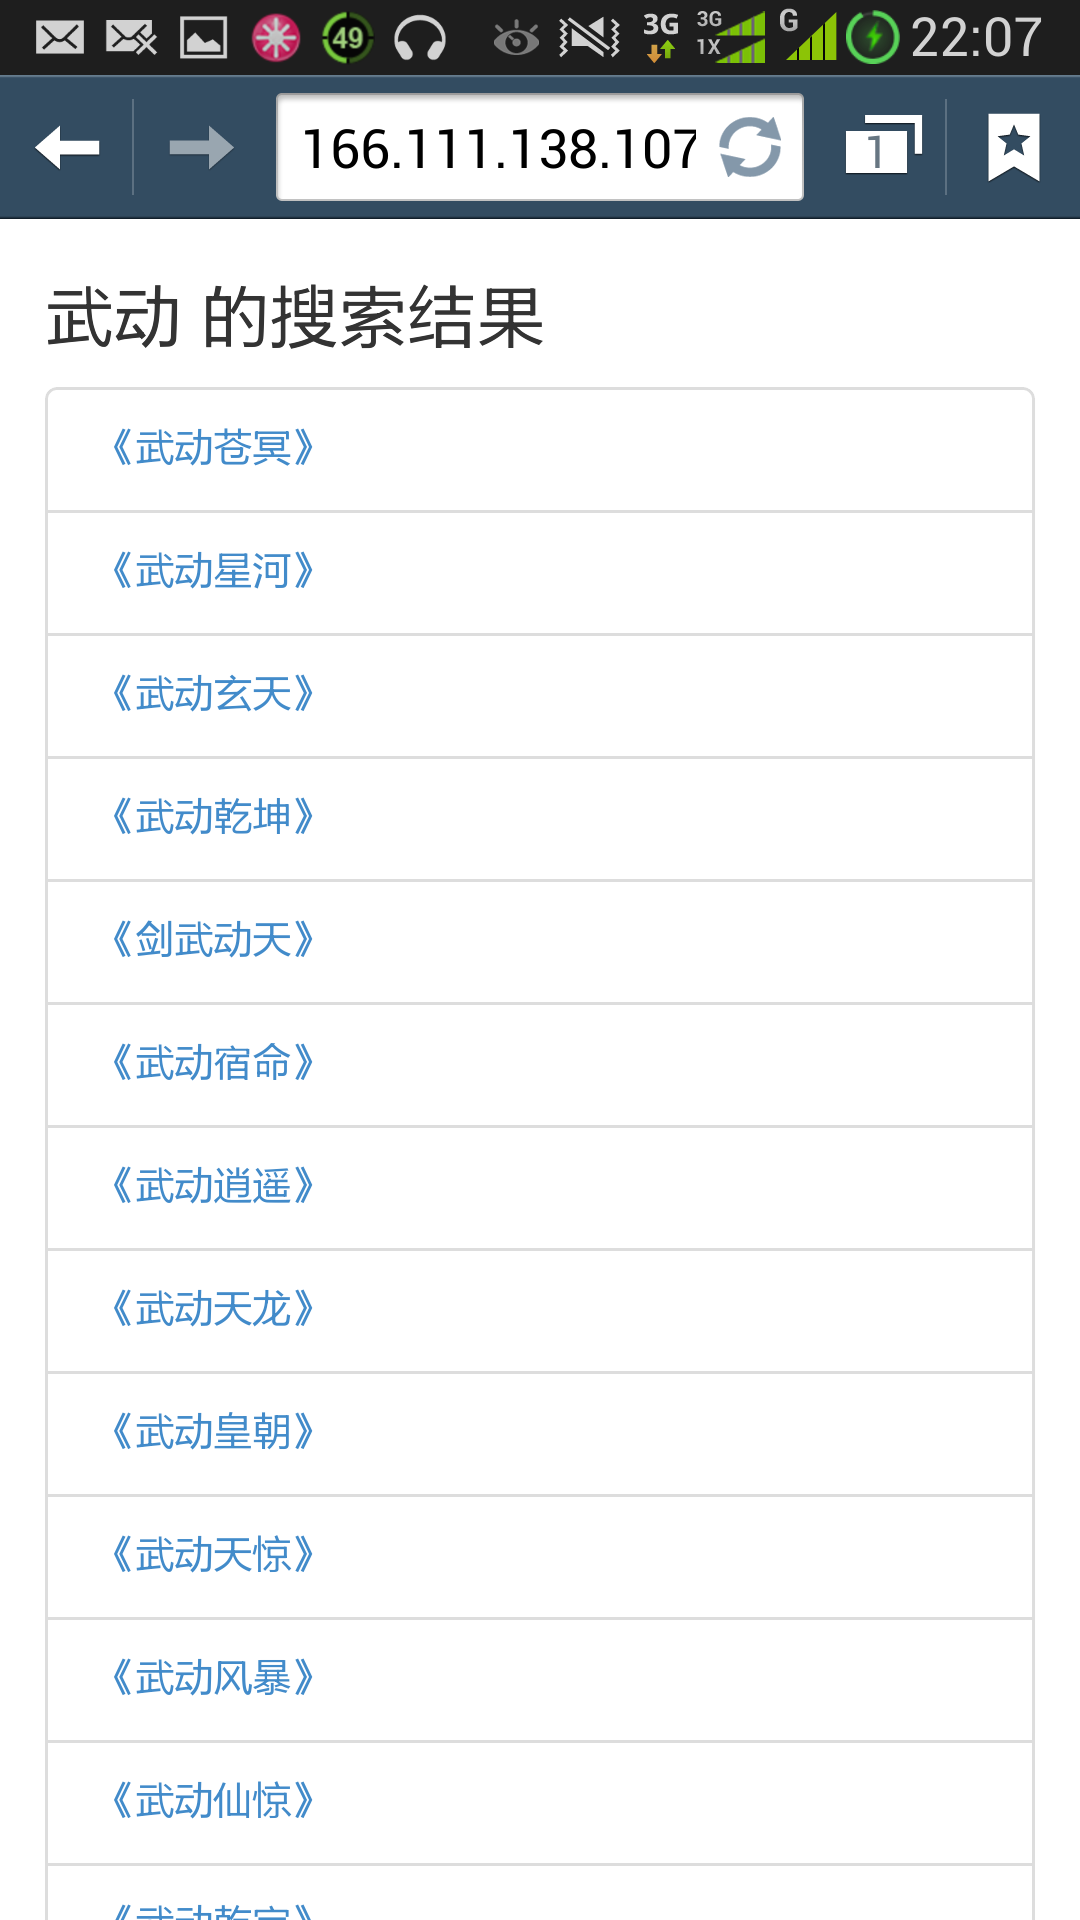
\includegraphics[width=\linewidth]{images/results.png}\\\centering{(b) Click a result to start downloading.}}
}
\vspace{0.5em}

Novels are retrived from multiple source sites, results from all source sites that has this novel will appear on the result list. Click a result will start downloading either a txt or a rar file directly, without any redirect to the source site and time wasted on figuring out the location of download link.
}

%%%%%%%%%%%%%%%%%%%%%%%%%%%%%%%%%%%%%%%%%%%%%%%%%%%%%%%%%%%%%%%%%%%%%%%%%%%%%%
\headerbox{Implementation}{name=results,column=1,span=1,row=0}{
  %%%%%%%%%%%%%%%%%%%%%%%%%%%%%%%%%%%%%%%%%%%%%%%%%%%%%%%%%%%%%%%%%%%%%%%%%%%%%%
NovelSearch's workflow is as follows
\begin{itemize}
\item User search on the web frontend
\item Web backend received search request
\item For every source site
\begin{itemize}
	\item Search the user request
	\item Find out download link
\end{itemize}
\item Gather results
\item Show results to user
\end{itemize}

For every source site, we wrote corresponding \emph{fetcher} to find download link by search keyword automatically. To add a source site, just add a fetcher for that site.

NovelSearch is wrote in Python, with Bootstrap for frontend, Flask as backend and BeautifulSoup as Html parser.
}

\headerbox{Project Site}{name=site,column=1,below=results}{
NovelSearch is currently serving on \url{166.111.138.107:13001}, try it by yourself!
}

\headerbox{Conclusion}{name=conclusion,column=1,below=site}{
We demonstrated NovelSearch, which can download a novel with only one input and one click. NovelSearch is much simpler to use than alternative solutions, as well as friendly to mobile devices.
}

\headerbox{Acknowledgement}{name=ack,column=1,below=conclusion}{
This is a course project for \emph{Software as a Service} in Tsinghua University. We thank our instructor Jie Tang for his excellent course.
}

\end{poster}

\end{document}

